%\section{Introduction/Motivation}
\subsection*{20. April 2020}
Was ist Measurement überhaupt?\\
Es geht darum mathematisch zu beschreiben
\begin{itemize}
    \item \emph{Was} wir messen?
    \item \emph{Worin} wir messen?
    \item \emph{Wie} wir messen?
\end{itemize}

\begin{example}
    Wir wählen drei Städte Q-Town, T-Town und P-Town (Also eine Menge mit drei Punkten im $\R^2$, die irgendwie erreichbar sind, bzw. die irgendwie verteilt im $\R^2$ sind). Die Frage ist nun wie wir die Entfernung zwischen den drei Städten messen könnten?
\end{example}
Was ist Measurement überhaupt?\\
Es geht darum mathematisch zu beschreiben
\begin{itemize}
    \item \emph{Was} wir messen?
    \item \emph{Worin} wir messen?
    \item \emph{Wie} wir messen?
\end{itemize}

\begin{example}
    Wir wählen drei Städte Q-Town, T-Town und P-Town (Also eine Menge mit drei Punkten im einer Ebene, die irgendwie erreichbar sind, intuitive ordnet wird von uns aber schon eine messbare Struktur angenommen, dass werden wir uns aber später nochmal überlegen, so stay tuned!). Die Frage ist nun wie wir die Entfernung zwischen den drei Städten messen könnten?
\end{example}
\begin{example}
    Nochmal genauer:
    \begin{itemize}
        \item Vektor(P-Town,T-Town) = (100 km East, 300km, North)
        \item Vektor(T-Town,Q-Town) = (200 km West, 100km, South)
        \item Vektor(T-Town,P-Town) = (100 km West, 200km, North)
        \item Vektor(T-Town,P-Town) = (100 km West, 300km, South)
    \end{itemize}
    \emph{Was} messen wir? Natürlich müssen wir die \emph{Städte-Paare} messen.\\
    \emph{Worin} messen wir? ``Quantifizierte Paare von Himmelsrichtungen'' (East-West, North-South)
\end{example}
\subsection*{21. April 2020}
%\todo[inline]{Put reference here for lecture 12 May 2020! fpr $\G_p$ definition!}
\begin{definition}[logistische Action Network]
    Das \emph{logistische Action Network} auf Menge $P$ ist gegeben durch
    \begin{itemize}
        \item $\G_P := (G_p, \ast, \id) \mit$
        \item $G_p := (P, P\times P, \id_{P\times P})\und$
        \item einem Produkt, nennen wir "Weglassprodukt", es ist definiert durch
        \begin{align*}
            (p,t)\ast (t,q) := (p,q) \quad \forall p,t,q \in P\\
            \text{sowie } \id \colon P \to P \times P \mit p \mapsto (p,p).
        \end{align*}
    \end{itemize}
\end{definition}
$$
        (p,t)\ast (t,q) = (p,q)\\ \quad
        \begin{tikzcd}[ampersand replacement=\&]
        q                                             \& t \arrow[l, "{(t,q)}"'] \\
        p \arrow[u, "{(p,q)}"] \arrow[ru, "{(p,t)}"'] \&      
    \end{tikzcd}\\ \quad\text{\emph{Was} messen wir? Punktepaare!}
$$
Dabei finden wir für jeden Punkt in $P$ genau eine Identitätsloop (ID-Loop) $\id$. Also zum Beispiel für $p$, die Identität $\id(p)=(p,p)$. \todo[inline]{Is this part of the definition?}
\begin{problem}
    Sei $\id(p) = (p,p)$ gegeben, was ergibt sich aus
    \begin{itemize}
        \item $\id(p)\ast (p,q) =$ ? % (p,q)
        \item $(p,q)\ast \id(q) =$ ? % (p,q)
        \item $(p,q)\ast (q,p) =$ ? % \id(p)
    \end{itemize}
\end{problem}
\begin{definition}[Weglass-Produkt]
    Wir definieren eine Abbildung $\ast \colon P^2 \times P^2 \to P^2$ durch
    \begin{align*}
        (p,t)\ast (t,q) = (p,q)
    \end{align*}
    wobei wir $\ast$ das \emph{Weglass-Produkt} nennen.
\end{definition}
Messbereiche (Worin messen wir!)
\begin{itemize}
    \item $\N_{\add} =(\N,+,0)$, wobei $\N = \set{0,1,2,\dots}$
    \item $\Z_{add} = (\Z,+,0)$, wobei $\Z = \N \cup \N^{-1}\cup \{0\}$, hier ist $\N^{-1} = \set{a \in \N \mid a^{-1} = -a}$. Okay besserer Weg geht über Äquivalenzrelation (Details könnten später hinzugefügt werden, wenn nötig!)\todo[inline]{thats mathemtically not good formulated.}
    \item $\Z^2_{add} = (\Z^2, +,0)$, hierbei $\Vec{0} = (0,0)$ und Operation $(m_1,n_1) + (m_2,n_2) := (m_1+n_1,m_2,n_2)$
    \item Das sind alles Beispiele für additive Monoide.
\end{itemize}
Nun definieren wir noch eine Abbildung $\vect$, du uns die Frage ``wie wir messen'' beantwortet.
\begin{definition}
    Sei $\vect \colon P \times P \to \Z^2$, also gilt
    \begin{align*}
        \vect(p,t) + \vect(t,q) &= \vect(p,q)\\
        &= \vect(p,t) \ast \vect(t,q)
    \end{align*}
    Also gehen wir den Graph entlang und messen die Abstände zwischen den Punkten mit $\vect$. (``Bild der Verkettung (semantisch $\ast$) ist Verkettung (semantisch +) der Bilder.'')
\end{definition}
\todo[inline]{Figure out how to draw!}
\begin{example}\mylinebreak\\
    \begin{minipage}{.5\textwidth}
        \todo[inline]{figure out how to draw it}
	\begin{center}
		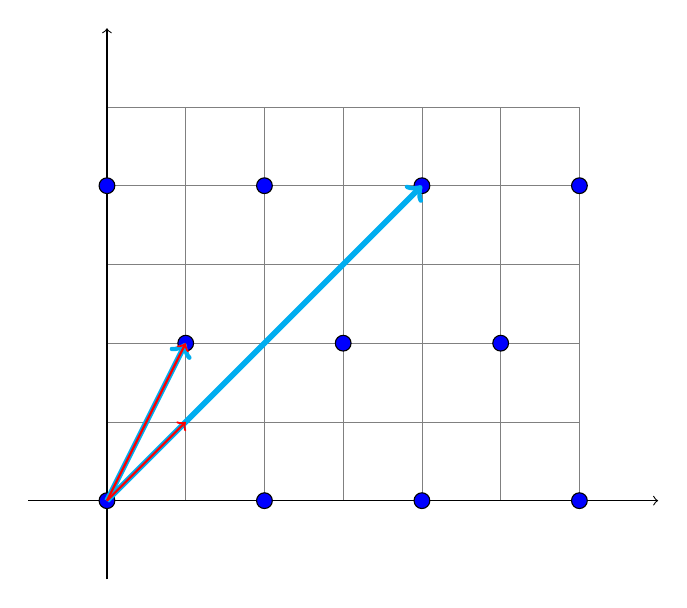
\begin{tikzpicture}
		\draw[help lines, line width=.2pt, step=1] (0,0) grid (6,5);
		\draw[->] (-1,0) -- (7,0);
		\draw[->] (0,-1) -- (0,6);
		\draw[fill=blue] (0,0) circle (0.1);
		\draw[fill=blue] (2,0) circle (0.1);
		\draw[fill=blue] (4,0) circle (0.1);
		\draw[fill=blue] (6,0) circle (0.1);
		\draw[fill=blue] (0,4) circle (0.1);
		\draw[fill=blue] (2,4) circle (0.1);
		\draw[fill=blue] (4,4) circle (0.1);
		\draw[fill=blue] (6,4) circle (0.1);
		\draw[fill=blue] (1,2) circle (0.1);
		\draw[fill=blue] (3,2) circle (0.1);
		\draw[fill=blue] (5,2) circle (0.1);
		\draw[->, cyan, line width=2pt] (0,0) -- (1,2);
		\draw[->, cyan, line width=2pt] (0,0) -- (4,4);
		\draw[->, red, thick] (0,0) -- (1,2);
		\draw[->, red, thick] (0,0) -- (1,1);
		\end{tikzpicture}
	\end{center}
    \end{minipage}%
    \begin{minipage}{.45\textwidth}
        \begin{itemize}
        \item $\vect(p,q) = (2,1)$
        \item $\vect(t,q) = (-1,1)$
        \item $\vect(p,q) = (1,2)$
        \end{itemize}
    \end{minipage}
\end{example}
\begin{remark}
    $(p,q)$ heißt auch ``syntaktischer Vektor'' (von $p$ nach $q$) für $p,q \in P$
\end{remark}
\subsection*{27. April 2020}
\paragraph{Zusammenfassung}
Das \emph{Was} ich messe ist im vorangegangen Fall ein \emph{logistisches Aktionsnetzwerk}.
\begin{definition}
Ein logistisches Aktionsnetzwerk auf einer Menge $P$ ist gegeben durch
    \begin{enumerate}
        \item $\G = (G_P, \ast, \id)$ mit Netzwerk
        \item $G_P = (P, P\times P, \id_{P \times P})$ mit
        \begin{align*}
            (p,q) := (p,t) \ast (t,q) \quad p,t,q \in P\quad \text{Weglass-Produkt}\\
            \id \colon P \to P \times P \mit p \mapsto (p,p) \quad \text{ID-Map}
        \end{align*}
    \end{enumerate}
\end{definition}
\begin{remark}
    \begin{itemize}
        \item $(p,q)$ heisst auch ``syntaktischer Vektor'' (von $p$ nach $q$) für $p,q \in P$.
        \item $\id(p) = (p,p)$ heisst der ID-Loop zum ``Knoten'' (Punkt) $p \in P$ in $\G_P$.
    \end{itemize}
\end{remark}

WORIN messe ich?

\begin{definition}[additives Monoid]
    Wir haben den additiven Monoid als Tripel $(\Z^2, +, \Vec{0})$ bezeichnet als $\Z^2_{\add}$ mit $\Vec{0} := (0,0)$. Mit der Verknüpfung $(x_1,y_1)+(x_2,y_2):= (x_1+y_1,x_2+y_2)$ für alle $x_1,x_2,y_1,y_2 \in \Z$.
\end{definition}
WIE messe ich ist mittels einer Abbildung
\begin{definition}
    Die ``vektoriellen Abbildung'' $\vect$ sei definiert durch
    \begin{align*}
        \vect \colon P \times P \to \Z^2
    \end{align*}
    \begin{enumerate}
        \item $\vect(\id(p)) = \vec{0} = 0$ für alle $p \in P$
        \item $\vect((p,t)\ast (t,q)) = \vect(p,t) + \vect(t,q)$ für alle $p,t,q \in P$.
    \end{enumerate}
\end{definition}
\begin{remark}
    $P\times P$ ist die Menge der \emph{syntaktischen} Vektoren, $\Z^2_{\add}$ ist der Monoid der \emph{semantischen} Vektoren im "MEASUREMENT SETUP" $(\G_P. \Z^2_{\add}, \vect)$
\end{remark}
\paragraph{Was ist ein Measurement Setup?}\mylinebreak\\
Nun verallgemeineren wir das noch zu
\begin{definition}[Measurement Setup]
    Es ist definiert als Tripel $\Measure = (\G, \M, \Delta)$ bestehend aus einem Aktionsnetzwerk $\G$, einem Monoid $\M$ und einer funktoriellen Abbdildung $\Delta$.
\end{definition}
\begin{remark}
    \begin{itemize}
        \item \emph{WAS} ich messe, ist $\G$.
        \item \emph{WORIN} ich messe, ist $\M$.
        \item \emph{WIE} ich meese, ist (mittels) $\Delta$.
    \end{itemize}
\end{remark}
\paragraph{Was ist ein Aktionsnetzwerk (ANW)?}
\begin{definition}[(Aktions) Netzwerk]
    Ein \emph{Netzwerk} ist Tripel $G = (V,E,\rho)$ bestehend aus zwei Mengen $V,E$, sowie $\rho \colon E \to V\times V = V^2$ mit $e \mapsto (\sigma e,\tau e)$.
    Setze $\sigma := \tau_1 \circ \rho \nd \tau = \tau_2 \circ \rho$, d.h. $\rho e = (\sigma e, \tau e)$.
\end{definition}
\todo[inline]{Find out where to put this little prop?}
\begin{satz}
    Sei $G = (V,E,\rho)$ ein Netzwerk, wenn $\ast$ assoziativer Operator, und $\id$ neutrales Element ist, dann ist $\G = (G,\ast, \id)$ ein Aktionsnetzwerk.
\end{satz}
\begin{proof}
    Einfaches nachrechnen. \todo[inline]{einfach mal machen ...}
\end{proof}
Ein ANW ist ein Tripel $\G = (G,\ast, \id)$ bestehend aus einem \emph{Netwerk} $G$ bestehend aus ``Zuständen'', ``Knoten'', ``Aktionen'' als ``Knoten'' und einer Abbildung, 
\begin{itemize}
    \item die jeder Kante ihre Anfangs-Endknotenpaar zugeordnet
        $$
        \begin{tikzcd}
            \sigma e \arrow[r, "e", bend left] & \tau e
        \end{tikzcd} \qquad\rho e = (\sigma e , \tau e)
        $$
    \item einer Abbildung $\ast$, die bestimmte Aktionen miteinander verkettet
        $$
        \begin{tikzcd}                                        & \bullet \arrow[rd, "b", bend left] &         \\
            \bullet \arrow[ru, "a", bend left] \arrow[rr, "a \ast b", bend right] &                                    & \bullet
        \end{tikzcd} \qquad
        \begin{tikzcd}
            p \arrow["\id(p)", loop, distance=2em, in=40, out=110]
        \end{tikzcd}
        $$
    \item eine ``ID-Loop'' Abbildung $\id$, die jedem Knoten seinen ID-Loop $\id(p)$ zuordnet.
\end{itemize}
\begin{interpret}
    \begin{itemize}
        \item $V$ ist die ``Knotenmenge'' (engl.: Knoten $\to$ Vertex oder Node).
        \item $E$ ist die ``Kantenmenge'' oder auch ``Pfeilmenge''. (engl. Kante $\to$ Edge, Pfeil $\to$ Arrow), $\rho$ ist die Strukturabbildung von $G$. Und das sieht dann so aus
        $$
        \begin{tikzcd}
            \sigma e \arrow[r, "e", bend left] & \tau e
        \end{tikzcd} \qquad\rho e = (\sigma e , \tau e)
        $$
        Es gilt $\rho e = (\sigma e, \tau e)$. Dabei ist $\sigma e$ der \emph{Source node of edge $e$} und $\tau e$ der \emph{Target node of edge $e$}.
    \end{itemize}
\end{interpret}
\begin{definition}\label{def_action_network}
    Ein Tripel $\G = (G, \ast, \id)$ ist \emph{Aktionsnetzwerk}, falls $G = (V,E,\rho)$ ein \emph{Netzwerk} ist und
    \begin{align*}
        \ast\colon E^{\Gen{2}} \to E
    \end{align*}
    eine Abbildung ist sowie
    \begin{align*}
        \id \colon V \to E
    \end{align*}
    eine Abbildung derart ist, dass gilt:
    $$
        \begin{tikzcd}                                        & \bullet \arrow[rd, "b", bend left] &         \\
            \bullet \arrow[ru, "a", bend left] \arrow[rr, "a \ast b", bend right] &                                    & \bullet
        \end{tikzcd} \qquad
        \begin{tikzcd}
            p \arrow["\id(p)", loop, distance=2em, in=40, out=110]
        \end{tikzcd} \qquad
        \begin{tikzcd}
            & \bullet \arrow[rr, "b \ast c"] \arrow[rd, "b"] &                         & \bullet \\
            \bullet \arrow[ru, "a"] \arrow[rr, "a \ast b"] \arrow[rrru, "(a \ast b) \ast c = a\ast (b \ast c)", bend left=49] &                                                & \bullet \arrow[ru, "c"] &        
        \end{tikzcd} \qquad
        \begin{tikzcd}
            \sigma e \arrow[r, "e"] \arrow["\id(\sigma e)", loop, distance=2em, in=40, out=110] & \tau e \arrow["\id(\tau e)", loop, distance=2em, in=40, out=110]
        \end{tikzcd}
    $$
\end{definition}
\subsection*{28. April 2020}
\paragraph{Wie kann MEASUREMENT mathematisch formalisiert werden?}
Durch ein \emph{Measurement Setup} wird de Frage beantwortet.
\begin{definition}[Measurement Setup]
    Ein \emph{Measurement Setup} besteht aus einem Tripel $\Measure = (\G, \M, \Delta)$ mit 
    \begin{itemize}
        \item \emph{Aktionsnetzwerk} $\G$ (Was ich messe)
        \item \emph{Monid} $\M$ (Worin ich messe)
        \item \emph{funktorieller Abbildung} $\Delta$ bezüglich $(\G,\M)$ funktoriell (Wie ich messe)
    \end{itemize}
\end{definition}
\paragraph{Was ist ein Aktionsnetzwerk?}
\begin{definition}
    Ein Aktionsnetzwerk ist ein Tripel $\G = (G,\ast, \id)$ bestehend aus
    \begin{enumerate}
        \item Netzwerk $G = (E,V,\rho)$, dabei war $\rho \colon E \to V \times V$
        \item Kantenabbildung $\ast$
        \item ID-Loop Map, bezeichnet mit $\id$, so dass die zwei Axiome, das Verkettungsaxiom und das Neutralitätsaxiom erfüllt sind.
    \end{enumerate}
\end{definition}
\begin{example}
    In der Beschreibung von ``Vernetzung'' ist der Begriff des Netzwerkes sehr zentral. Hier mal einige Beispiel aus dem Leben:
    \begin{itemize}
        \item \emph{Internet}
        \item \emph{soziale Netzwerke}
        \item \emph{Navigationssysteme}
    \end{itemize}
\end{example}
\paragraph{Was bringt uns das mathematisch?}\mylinebreak\\
Wir wollen Prozesse und Strukturen innerhalb und auch ausßerhalb der Mathematik \emph{geometrisieren} und danach abstrakte beschreibungen mit Anschauung und besserer Intuition versehen.
\begin{remark}
    Die Netzwerk-Sicht erlaubt und dabei ``Sozial Brain'' (``Netzworking Brain'') einzuschlaten - das übrigens sehr groß ist und auch gerne mtmacht, wenn es um Präsentation von Information geht.
\end{remark}
Nochmal etwas genauer zum Begriff ``Pfeil'':
\paragraph{Was ist ein Pfeil?}
$$
\begin{tikzcd}
                            & \quad \\
\quad \arrow[ru, bend left] &      
\end{tikzcd} 
\begin{tikzcd}
                                                       & \quad \\
\quad \arrow[ru, Rightarrow, bend left] &      
\end{tikzcd}
$$
Zunächst ist ein Pfeil ein ``archetypisches Symbol'', das in der Geschichte der Menschheit weit zurückreicht. In der ``Semantik''(Lehre der zeichen und ihrer Bedeutung) wird seine vielfältige Sicht erörtert. Eine einefache Modellierung besagt, dass es Pfeil einen ``Anfangspunkt'' mit einem ``Endpunkt'' verbindet, oder anders gesagt, einem Anfangs- und einem Endpunkt besitzt
$$
\begin{tikzcd}
    \bullet \arrow[r, bend left] & \bullet
\end{tikzcd}
$$
\paragraph{Was ist ein Netzwerk?}
\begin{remark}
    In der Mathematik wird hierfür der Begriff ``gerichteter Multigraph'' verwendet.
\end{remark}
\begin{example}
    $$
    \begin{tikzcd}
        \bullet \arrow[loop, distance=2em, in=200, out=270] \arrow[r, bend left=49] \arrow[r, bend right] & \bullet \arrow[r] & \bullet \arrow[ll, bend left=49]
    \end{tikzcd}
    $$
\end{example}
\begin{remark}
    Ein Netzwerk heisst \emph{$n$-knotig}, falls seine Knotenmenge $n$-elementig ist (wobei $n \in \N$ sei).
\end{remark}
Wir geben folgende algemeine Definition
\begin{definition}[mathematische Defintion Netzwerk]
    Ein \emph{Netzwerk} ist geklärt als Tripel $G = (V,E,\rho)$ bestehend aus zwei Mengen $V$ und $E$ sowie einer Abbildung $\rho\colon E \to V\times V$.
\end{definition}
\begin{interpret}
    \begin{itemize}
        \item $V$ Menge von ``Konten'' in $G$ (english: ``vertices'', ``nodes'')
        \item $E$ Menge von ``Kanten'' bzw. ``Pfeilen'' in $G$ (english: ``edges'', ``arrow'')
        \item $\rho$ ist die sogennante ``Struktur-Abbildung'' von $G$
    \end{itemize}
\end{interpret}
Weitere Interpretation
\begin{interpret}
    Die Abbildung $\rho$ induziert zwei Abbildungen $\sigma := \pi_1 \circ \rho$ ist die ``Projektion von $\rho$ auf die erste Komponente'' und $\tau := \pi_2 \circ \rho$ ist die ``Projektion auf die zweite Komponente''. Also gilt
    \begin{align*}
        \rho e = (\sigma e, \tau e)
    \end{align*}
    Für jede Kante $e$ in $G$ gilt:
    $$
    \begin{tikzcd}
        \sigma e \arrow[r, "e", bend left] & \tau e
    \end{tikzcd}
    $$
    Dabei $\sigma e$ heisst der \emph{Anfangsknoten} (``source node'') von $e$ in $G$ und $\tau e$ heisst der \emph{Endknoten} (``target node'') von $e$ in $G$.
\end{interpret}
\begin{example}
    Ein Netzwerk (mathematisch wohldefiniert):
    $$
    \begin{tikzcd}
        p \arrow[r, "a", bend left=49] \arrow[r, "b"] \arrow["e"', loop, distance=2em, in=190, out=120] & t \arrow[r, "c"] & q \arrow[ll, "d", bend left]
    \end{tikzcd}
    $$
    \begin{itemize}
        \item $G = (V,E,\rho)$
        \item $V= \set{p,q,t}$
        \item $E = \set{a,b,c,d,e}$ und $\rho$ definiert via
        \begin{center}
            \begin{tabular}{c||c|c|c|c|c}
                %\hline
                $x$ & $a$ & $b$ & $c$ & $d$ & $e$ \\ \hline 
                $gx$ & $(p,t)$ & $(p,t)$ & $(t,q)$ & $(q,p)$ & $(p,p)$\\ %\hline 
            \end{tabular}
        \end{center}
    \end{itemize}
\end{example}
\begin{notation}[Algemeine Notation]
    \begin{itemize}
        \item $\N$ bezeichne die Menge der natürlichen Zahlen \emph{beginnend} mit 0, also $\N = \set{0,1,2,\dots}$. Dann bezeichnet $\N_+$  also die Menge der positiven natürlichen Zahlen, damit $\N_+ = \set{1,2,\dots}$.
        \item Für $n \in \N$ sei $[n] := \set{1,\dots,n}$, d.h. $[n] = \set{m \in \N_+ \mid m \le n}$ und ausserdem sei $\emph{n}:= \set{1, \dots, n-1}$, d.h. $\emph{n} := \set{m \in \N \mit m < n}$
    \end{itemize}
\end{notation}
Zentral ist hier der Begriff \emph{Pfades} (engl. path) in einem Netzwerk.
\begin{definition}[Pfad der Länge $n$, Menge aller Pfade]
    Sei $G = (V,E,\rho)$ ein Netzwerk (mit induzierten Abbildungen $\rho$ und $\tau$) und sei $n \in \N_+$. 
    \begin{itemize}
        \item Ein \emph{Pfad der Länge $n$} in $G$ erklärt als $n$-Tupel $(e_1, \dots, e_n) \in E^n$ mit $\tau e_i = \sigma e_{i+1}$ für alle $i \in [n-1]$.
        \item Es bezeichne $E^{\Gen{n}}$ die Menge aller Pfade der Länge $n$ in $G$.
        \item Ferner sei 
        \begin{align*}
            E^{\Gen{+}} := \bigcup_{n \in \N_+} E^{\Gen{n}}
        \end{align*}
        die Menge aller \emph{Pfade} in $G$.
    \end{itemize}
    \emph{Beachte:} Hier ist noch kein Pfad der Länge 0 enhalten, diese muss noch konstruiert werden. (Meist sind diese aber, die jeweiligen ID-Loops zu einem Element $v \in V$)\todo[inline]{how to write this down in a proper way?}
\end{definition}
\begin{example}
    \begin{itemize}
        \item Pfad der Länge 1 (wir identifizieren $E^1$ mit $E$)
        $$
        \begin{tikzcd}
            \bullet \arrow[r, "e", bend left] & \bullet
        \end{tikzcd}
        $$
        \item $\tau e_1 = \tau e_2$ Pfad der Länge 2
        $$
        \begin{tikzcd}
            \bullet \arrow[r, "e_1"] & \bullet \arrow[r, "e_2"] & \bullet
        \end{tikzcd}
        $$
        \item Pfad der Länge 3 (hier ist $\tau e_1 = \sigma e_2$ und $\tau e_2 = \sigma e_3$)
        $$
        \begin{tikzcd}
            \bullet \arrow[r, "e_1"] & \bullet \arrow[r, "e_2"] & \bullet \arrow[r, "e_3"] & \bullet
        \end{tikzcd}
        $$
        \item Pfad der Länge $n$ (hier ist $\tau e_1 = \sigma e_2$ und $\tau e_{n-1} = \sigma e_n$) \todo[inline]{Put generalization of length $n$, maybe still wrong}
        $$
        \begin{tikzcd}
            \bullet \arrow[r, "e_1"] & \bullet \arrow[r, "e_2"] & \dots \arrow[r, "e_n"] & \bullet
        \end{tikzcd}
        $$
    \end{itemize}
\end{example}
\begin{example}[Details]
    \begin{itemize}
        \item Sei $\Relat = (P,R)$ \emph{binäres Relat}, d.h. $P$ und $R$ sind Mengen mit $R\subseteq P \times P$, also "$R$ ist binäre Relation auf $P$". Dann ist $G\Relat := (P,R,\rho)$ mit 
        \begin{align*}
            \rho \colon R \to P\times P \mit (p,q) \mapsto (p,q)
        \end{align*}
        ein Netzwerk. Das sieht dann so aus
        $$
            \begin{tikzcd}
                p \arrow[r, "{(p,q)}"] & q
            \end{tikzcd}.
        $$
        \begin{remark}
            \begin{itemize}
                \item Wir sagen auch, dass ``$G\Relat$ das binäre Relat $\Relat$'' als Netzwerk (interpretiert) ist".
                \item Ein Netzwerk heisst \emph{dünn} (engl. ``thin''), falls seine Strukturabbildung \emph{injektiv} ist.
            \end{itemize}
            Es ist also $G\Relat$ stets ein dünnes Netzwerk.
        \end{remark}
        \item Sei $G=(V,E,\rho)$ Netzwerk. Dann ist
        \begin{align*}
            \Path(G) := G^{\Gen{+}} := (V, E^{\Gen{+}}, \rho^{\Gen{+}})
        \end{align*}
        mit $\rho^{\Gen{+}}(e_1, \dots, e_n) := (\sigma e_1, \tau e_n)$ für alle $(e_1, \dots, e_n) \in E^{\Gen{+}}$ (mit $n \in \N_+$) ein Netzwerk, das sogenannte \emph{Pfad-Netzwerk} (engl. ``path netzwerk'') zu $G$
        $$
        \begin{tikzcd}
            \sigma e_1 \arrow[r, "e_1"] & \bullet \arrow[r, "e_2"] & \bullet \arrow[r, "e_3"] & \tau e_3
        \end{tikzcd}
        $$
        \item Sei $A$ Menge (z.B. ein ``Alphabet'') und sei $\perp$ ein Symbol (welcher oft ``Bottom'' gennant wird). Dann 
        \begin{align*}
            \cloverleaf(A, \perp) := (\set{\perp}, A, \rho) \mit \rho \colon A \to \set{(\perp, \perp)}, a \mapsto (\perp, \perp)
        \end{align*}
        ein ``1-knotiges'' Netzwerk, das sogenannte \emph{Kleeblatt-Netzwerk} zu $(A,\perp)$ 
        $$
        \begin{tikzcd}
            \perp \arrow["a_1", loop, distance=2em, in=0, out=40] \arrow["a_3",loop, distance=2em, in=290, out=340] \arrow["a_2",loop, distance=2em, in=200, out=250]
        \end{tikzcd}
        $$
    \end{itemize}
\end{example}
\begin{remark}
    Ein Netzwerk heisst ``$n$-knotig'', falls seine Knotenmenge $n$-elementig ist (wobei $n \in \N$ sei).
\end{remark}
\paragraph{Zusammenfassung Netzwerk-Beispiele}
\begin{itemize}
    \item Jedes binäres Relat können wir als Netzwerk auffassen, denn ``binäre Relate liefern dünne Netzwerke''
    \item Zu jedem Netzwerk lässt sich das Pfad-Netzwerk betrachten, denn die Knoten des Pfad-Netzwerks sind gerade die Pfade, des zugrunde liegenden Netzwerkes, diese nennt man auch ``Meta-Kanten''.
    \item Zu jeder Menge gibt es ein 1-knotiges Kleeblatt-Netzwerk.
\end{itemize}
\paragraph{Was ist ein Aktionsnetzwerk?}\mylinebreak{}\\
Diese Frage beantworten wir jetzt mit der folgenden mathematischen Definition. (Vorab eine kleine \emph{Motivation}):
Aktionsnetzwerke sind Netzwerke, deren Kanten wir als \emph{Aktionen} auffassen, die eingeschränkt \emph{verkettbar} sind und ausserdem haben wir in jedem Knoten einen sogenannten ``ID-Loop'', die \emph{Passitivität} bzw. \emph{Neutralität} in jeweiligen Knoten beschreibt. Formal ist ein ``Aktionsnetzwerk'', wie folgt erhält man die Definition auf Seite \pageref{def_action_network}.
\begin{overview}[Ausblick]
Hier werden nochmal ein paar Fragen beantwortet:
    \begin{itemize}
        \item ``Netzwerk'' ist das Gleiche wie ``gerichteter Multigraph'' ($\compare$ als Begriff der Graphentheorie).
        \item ``Aktionsnetzwerk'' ist das Gleiche wie ``kleine co-variante Kategorie'' ($\compare$ Kategorientheorie).
        \item Struktur-respektierende Transformationen heissen ``Morphismen'' (griechisch: ``gestalt-respektierend ...'').
        \item Was ist allgemein eine struktur-respektierende Transformation? Informell gesagt, geht es hier um Abbildungen derart, dass gilt: ``Das Bild vom Blabla ist das Blabla vom Bild.''
        \item Für ``Aktionsnetzwerke'' ($\compare$ allgemein für ``Kategorien'') nennt man solche Morphismen auch ``Funktoren''.
        \item Eine struktur-respektierende Transformation zwischen ANWs nennen wir also ``Funktor''. Eine ``funktorielle Abbildung'' respektiert in gewisser Weise die Struktur. (Soweit sind wir im Moment noch nicht!) Die Begriffe ``Morphismen'' und ``Funktoren'' folgen demnächst!
    \end{itemize}
\end{overview}